\documentclass[a4paper,10pt]{article} 

\usepackage[utf8]{inputenc} 
%\usepackage[T1]{fontenc}

\usepackage{textcomp}           % Extra Symbole (Grad Celsius etc.)
\usepackage{amssymb,amsmath}    % Schöne Formeln (AMS = American Mathematical Society)
\usepackage{graphicx}           % Bilder und Seitenränder
\usepackage{subcaption}			% captions for subfigures
\usepackage{booktabs}           % Schönere Tabellen
\usepackage{colortbl}           % Farbige Tabellen

%\usepackage{tcolorbox}			% schöne bunte Boxen
\usepackage{mathtools}			% \mathclap für ordentliche \underbrace-			environments
\usepackage[left=2cm,right=2cm,top=2cm,bottom=2cm]{geometry}			% Pagelayout mit \newgeometry, \restoregeometry
\usepackage{float}
\usepackage{wrapfig}
\usepackage{enumitem}
\usepackage{float}
\usepackage{braket}
\usepackage{caption}
\usepackage[per-mode=reciprocal,output-decimal-marker={.},binary-units=true]{siunitx}
\usepackage[breaklinks=true,colorlinks=true,linkcolor=blue,urlcolor=blue,citecolor=blue]{hyperref} 
\usepackage{physics}
\usepackage{url}
\usepackage{subcaption}
\usepackage{calrsfs}
\DeclareMathAlphabet{\pazocal}{OMS}{zplm}{m}{n}

\graphicspath{{./img/}}

\newcommand{\dif}{\mathrm{d}}

\bibliographystyle{unsrtnat}

\renewcommand{\k}{\mathbf{k}}
\begin{document}
\begin{titlepage}
 \begin{center}
	\Large{Advanced laboratory class 3}
	\end{center}
	\begin{center}
	 \LARGE{\textbf{FP3 - SQUID}}
	\end{center}
	
	\begin{center}
	
	\large Marco \textsc{Canteri} \\
	marco.canteri@student.uibk.ac.at\\
	\large Maximilian \textsc{Münst} \\
	maximilian.muenst@student.uibk.ac.at
	\end{center}
	
	\begin{center}
	\vspace{1cm}
	Innsbruck, \today
	\vspace{1cm}
	\end{center}
	
	\begin{abstract}
    In the course of this experiment a look was taken at some basic properties of superconducturs and SQUIDs, like the current-voltage and the current-flux characteristics. Additionally, Shapiro-steps were observed from which the $e/h$-ratio can be calculated. Finally, the resistance of the SQUID was measured, dependent on the temperature. 
    \end{abstract}
    \vspace{1cm}
	
	\begin{center}
	
\includegraphics[scale=0.4]{img/uibk} 
	\end{center}

\end{titlepage}


\section{Introduction}
In most solid body physics courses one learns that the resistance of a substance is caused by electron scattering on obstacles like phonons, impurities in the lattice, or other electrons.\cite{grossmarx} This model predicts that the resistance decreases with decreasing temperature, but ultimately remains at a finite, non-zero value due to impurities in the lattice. 
However, in 1911 Heike Onnes discovered a drastic and unforeseen decrease in resistance of mercury at \SI{4.2}{\kelvin}, later terming the observed phenomenon superconduction. 
\begin{quote}
    Mercury has passed into a new state which, on account of its extraordinary electrical properties, may be called the superconductive state. \newline
    -- \textsc{Heike Kamerlingh Onnes}, according to \cite{grossmarx}
\end{quote} 
In 1933 Walther Meißner and Robert Ochsenfeld discovered that in addition to being perfect conductors, superconducting materials also are perfect diamagnets. Today, applications of superconduction range from Magnetic Resonance Imaging (MRI) in medicine to particle accelerators, where superconducting coils are used to generate powerful magnetic fields.\cite{grossmarx}

\section{Theoretical Background}

The theoretical introduction in this report is split into two parts, one being a general introduction to superconductivity, while the other one is about the Josephson Effect and its application in this experiment. The presented information us based on the ``Mr. SQUID''-manual \cite{skriptum} as well as the book ``\textit{Festkörperphysik}'' \cite{grossmarx}.

\subsection{Superconductivity}
Superconductivity is the property of a medium to conduct current without any resistance. It was first discovered in 1911, when Heike Onnes cooled down mercury below 4.2 K \cite{firstsuperconductor}, finding out that the resistance dropped to zero. Since this discovery, superconductivity has been discovered in many elements and media which resistance drops to zero below a particular critical temperature $T_c$. There are different ways to classify superconductors, the easiest one is to divide superconductors in low-$T_c$ and high-$T_c$ superconductors. Low temperature superconductors are material with a critical temperature below $30$ K, while high temperature superconductors have $T_c$ greater than 30 K.\\
Superconductors can lose their property of superconductivity not only with a change in temperature, but also with a change of magnetic field or current, this leads to a different classification of superconductors: type I and type II superconductors. The former has a critical external magnetic field $H_c$ and behaves as superconductor below this field. Type II superconductors have two different critical fields, and they behave differently in various regimes.\\
In this experiment we used a Yttrium barium copper oxide (YBCO) superconductor which is a high-$T_c$ superconductors, historically is also the first high-$T_c$ superconductors found with a critical temperature above 77 K, the boiling point of liquid nitrogen. Indeed the critical temperature of YBCO is around 90-94 K, depending of the compound and purity.\\
The theoretical description of superconductivity can be done in different ways, the first classical approach is the simplest description using London equations, a quantum mechanical formulation is the Ginzburg-Landau (GL) theory which describes the macroscopic properties of superconductors. However this theory is still phenomenological, the first microscopic model is the BCS theory which was able to describe superconductivity from a microscopic point of view and has the GL theory as a limit. The key idea of BCS theory is that at low temperatures electrons pair up and form Copper pairs, creating a bosonic condensate. This condensate must be described as a single entity with a wavefunction $\psi(\mathbf{r},\theta) = |\psi(\mathbf{r})| e^{i\theta}$, which is not normalized, but $|\psi(\mathbf{r},\theta)|^2 = n_e$, where $n_e$ is the number of electrons in the superconductive state. These theory predicts the behaviour of low temperature superconductors, but fails to describe high temperature superconductors, whose description is still an open problem.

\subsection{Josephson Effect and SQUID} % AC, DC Josephson effect & Shapiro steps, SQUID 

\subsubsection*{DC Josephson Effect}
The Josephson effect is caused by the long range quantum interaction in superconductors. The junction itself can be seen as a gap or barrier between two superconductors as is sketched in Fig. \ref{figure_josephson_junction}. In the Mr. SQUID \cite{skriptum} device, the junctions are grain boundary weak-link junctions. 

\begin{figure}[htp!]
    \centering
    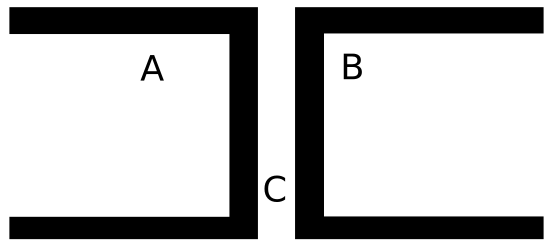
\includegraphics[width = 0.6 \textwidth]{josephson.png}
    \caption{Sketch of a Josephson junction. The wavefunctions with respective phases $\varphi_A$ and $\varphi_B$ interfere over the barrier C.}
    \label{figure_josephson_junction}
\end{figure}

The supercurrent flowing through the junction is dependent on the density of electron-electron pairs or Cooper pairs $n_{S,A}$ and $n_{S,B}$, the phases of the two macroscopic wave functions $\Psi_A$ and $\Psi_B$ and the properties of the junction. Assuming that the coupling is small, it follows that $\abs{\Psi_A}^2 = n_{S,A}$ and $\abs{\Psi_B}^2 = n_{S,A}$ remain approximately constant and should have the same value $n_{S}$. 
According to \cite{grossmarx}, the most general expression for the supercurrent density is then 
\begin{equation}
    J_S = q_S n_S(\vec{r},t) \big[ \frac{\hbar}{m_S} \nabla \Theta(\vec{r},t) - \frac{q_S}{m_S} \vec{A}(\vec{r},t) \big] = \frac{q_S n_S \hbar}{m_S} \vec{\gamma}(\vec{r},t)
\end{equation}
with $\vec{\gamma}(\vec{r},t) = \nabla \Theta - \frac{2 \pi}{\Phi_0} \vec{A}(\vec{r},t)$. It is fair to assume that the phase gradient in the barrier is big compared to the gradient in the superconductor. Assuming further that the phase gradient $\vec{\gamma}$ is constant over the small junction, one can introduce a gauge invariant phase difference $\phi(\vec{r}, t)$ as 
\begin{equation}
    \begin{split}
        \label{eq_phase}
        \varphi(\vec{r}, t) &= \int^B_A \vec{\gamma}(\vec{r},t) = \int^B_A \big[ \nabla \Theta - \frac{2 \pi}{\Phi_0} \vec{A}(\vec{r},t) \big] \dif \vec{l} \\
        &= \Theta_B(\vec{r}, t) - \Theta_A(\vec{r}, t) - \frac{2 \pi}{\Phi_0} \int^B_A \vec{A}(\vec{r},t) \dif \vec{l}
    \end{split}
\end{equation}

According to \cite{skriptum}, the supercurrent $I_S$ solely depends on the phase difference $\varphi$. Furthermore, the wave functions $\Psi_A$ and $\Psi_B$ have to be invariant under a phase change of a multiple of $2 \pi$. 
\begin{equation}
    I_S(\varphi) = I_S(\varphi + n 2 \pi)
\end{equation}
Also, if there is no supercurrent in the superconductor, the phase difference has to be $0$. Hence, one can write 
\begin{equation}
    I_S(\varphi = 0) = 0 = I_S( n 2 \pi).
\end{equation}
Combining these results leads to sinusodial dependence of the supercurrent $I_S$ on the phase difference $\phi$.
\begin{equation}
    I_S(\varphi) = I_C \sin(\varphi) + \underbrace{\sum^{\infty}_{m = 2} I_m \sin(m \varphi)}_{\approx 0}
    \label{first_josephson}
\end{equation}
Eq. \ref{first_josephson} is often referred to as the first Josephson equation. The higher order terms are often ignored as they are usually very small. 

The second Josephson equation can be calculated from the time derivative of Eq. \ref{eq_phase}, which is 
\begin{equation}
    \pdv{\varphi}{t} = \pdv{\Theta_B}{t} - \pdv{\Theta_A}{t} - \frac{2 \pi}{\Phi_0} \pdv{}{t} \int^B_A \vec{A}(\vec{r},t) \dif \vec{l}.
\end{equation}
Using the energy-phase relation form \cite{grossmarx}, which is given as 
\begin{equation}
    -\hbar \pdv{\Theta}{t} = \frac{1}{2 n_S} \Lambda \vec{J_S}^2 + q_S \phi + \mu,
\end{equation}
where $\Lambda = \frac{m_S}{n_S q_S^2}$ is the London coefficient, $q_S = -2 e$ is the charge of a Cooper pair, $\phi$ is a gauge scalar field and $\mu$ is the chemical potential. This yields the following expression:
\begin{equation}
    \pdv{\varphi}{t} = - \frac{1}{\hbar} \big( \frac{\Lambda}{2 n_S} \underbrace{[\vec{J}_S^2(B) - \vec{J}_S^2(A)]}_{ = 0} + q_S [\phi(B) - \phi(A)] + [\mu(B) - \mu(A)] \big) -  \frac{2 \pi}{\Phi_0} \pdv{}{t} \int^B_A \vec{A}(\vec{r},t) \dif \vec{l}
\end{equation}
Continuity requires that the currents at both sides of the junction are equal in size. This then leads to the second Josephson equation:
\begin{equation}
\pdv{\varphi}{t} = \frac{2 \pi}{\Phi_0} \int^B_A \big[ - \nabla \tilde{\phi} - \pdv{\vec{A}}{t} \big] \dif \vec{l} = \frac{2 \pi}{\Phi_0} \int^B_A \vec{E}(\vec{r},t) \dif \vec{l} = \frac{2 \pi}{\Phi_0} U,
\end{equation}
where $U$ is the voltage over the junction. It follows that the phase increases with time, resulting in 
\begin{equation}
    \varphi(t) = \varphi_0 + \frac{2 \pi}{\Phi_0} U t.
    \label{eq_josephson_2}
\end{equation}

\subsubsection*{AC Josephson Effect} % AC & Shapiro Steps
If one now adds an alternating current to the DC voltage $U = U_0 + U_1 \sin(\omega_1 t)$ in Eq. \ref{eq_josephson_2}, one gets 
\begin{equation}
    \varphi(t) = \varphi(0) + \frac{2 e U_0}{\hbar} t + \frac{2 e U_1}{\hbar \omega_1} \sin(\omega_1 t).
\end{equation}
This expression can now be inserted into the first Josephson equation, which yields 
\begin{equation}
    I_S(\varphi) = I_C \sin \big( \varphi(0) + \frac{2 e U_0}{\hbar} t + \frac{2 e U_1}{\hbar \omega_1} \sin(\omega_1 t) \big). 
\end{equation}
Using the first order Bessel function $\pazocal{J}$, one can write
\begin{equation}
    J_S(t) = J_C \sum^{\infty}_{n = 0} \pazocal{J}_n \big[ \frac{2 e U_1}{\hbar \omega_1} \big] \underbrace{\sin \big( \varphi(0) + \frac{2 e U_0}{\hbar} t \pm n \omega_1 t \big)}_{= const \Leftrightarrow U_0 = n \frac{\hbar \omega_1}{2e}}.
\end{equation}
Since one usually measures the DC components in the experiment, one has to find the DC voltage at which the sine becomes time-independent. This is true for $U_0 = n \frac{\hbar \omega_1}{2e}$. If one measures the $I$-$V$ characteristic of a Josephson junction, one will see steps in the curve. The height of the steps is determined by the amplitude of the alternating current $U_1$ and the corresponding Bessel function $\pazocal{J}_n$. They are often called Shapiro steps.

\subsubsection*{Superconducting QUantum Interference Device - SQUID}
A simple circuit diagram of a SQUID is displayed in Fig. \ref{fig_squid}. It shows that the Josephson junctions are set up in a parallel way and are connected with superconducting material. Assuming that the critical current $I_C$ is equal for both junctions, one can use the phase-current relation from \cite{grossmarx}, which says that the currents in then junctions can be expressed as $I_{S,1}=I_C \sin(\varphi_1)$ and $I_{S,2} = I_C \sin(\varphi_2)$.
\begin{figure}[htp!]
    \centering
    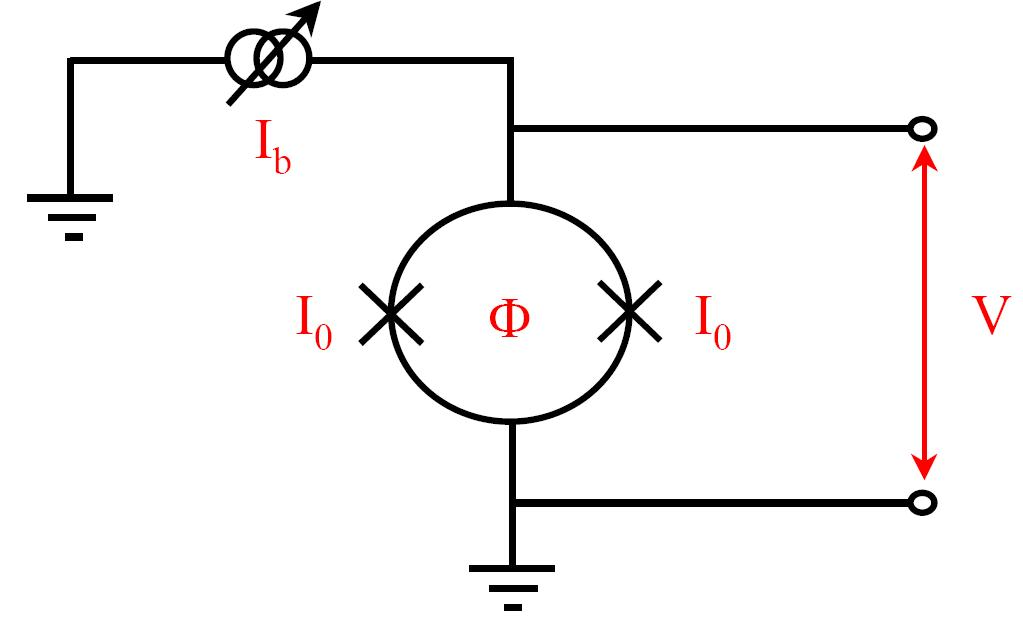
\includegraphics[width = 0.6 \textwidth]{SQUID_IV.jpg}
    \caption{Schematic of a DC SQUID, taken from \cite{squid_circuit}. An input bias current $I_b$ produces a voltage over the two parallel arranged Josephson junctions, through which a current $I_0$ is passing. If one now adds a magnetic flux $\Phi$ through the SQUID, an additional current $I_S$ is induced, which is running circular in the SQUID, adding to the bias current in the Josephson junctions. This induced current reduces the critical current of the SQUID.}
    \label{fig_squid}
\end{figure}
Using Kirchhoff's law and the addition theorems, one can write the total current as 
\begin{equation}
    \label{eq_continuity}
    I_S = I_{S,1} + I_{S,2} = 2 I_C \cos(\frac{\varphi_2 - \varphi_1}{2}) \sin(\frac{\varphi_1 + \varphi_2}{2})
\end{equation}
According to \cite{grossmarx}, one can further argue that in the total phase change across the ring, the phase change in the superconductor is negligible compared to the change in the Josephson junctions. Therefore, one can reach the following equation using Eq. \ref{eq_phase}. 
\begin{equation}
    \varphi_1 - \varphi_2 = - \frac{2 \pi}{\Phi_0} \underbrace{ \oint \vec{A} \dif \vec{l} }_{= \Phi}
\end{equation}
Here $\Phi$ is the flux through the SQUID. Inserting this into Eq. \ref{eq_continuity} leads to 
\begin{equation}
    I_S^\mathrm{max} = 2 I_C \cos(\frac{\pi \Phi}{\Phi_0}) \sin(\varphi_1 + \frac{\pi \Phi}{\Phi_0}) \stackrel{\Phi = \Phi_\mathrm{ext}}{=} 2 I_C \abs{\cos \big( \frac{\pi \Phi_\mathrm{ext}}{\Phi_0} \big)}.
\end{equation}
This equation finally shows the critical maximum the supercurrent can reach when a magnetic field is applied on the SQUID. $I_C$ in this equation means the critical current per junction, which is half the critical current of the SQUID. 

\section{Experimental Setup}

%\section{Theory}
%\subsection{Superconductivity}
%Superconductivity is the property of a medium to conduct current without any resistance. It was first discovered in 1911, when Heike Onnes cooled down mercury below 4.2 K \cite{firstsuperconductor}, finding out that the resistance dropped to zero. Since this discovery, superconductivity has been discovered in many elements and media which resistance drops to zero below a particular critical temperature $T_c$. There are different ways to classify superconductors, the easiest one is to divide superconductors in low-$T_c$ and high-$T_c$ superconductors. Low temperature superconductors are material with a critical temperature below $30$ K, while high temperature superconductors have $T_c$ greater than 30 K.\\
%Superconductors can lose their property of superconductivity not only with a change in temperature, but also with a change of magnetic field or current, this leads to a different classification of superconductors: type I and type II superconductors. The former has a critical external magnetic field $H_c$ and behaves as superconductor below this field. Type II superconductors have two different critical fields, and they behave differently in various regimes.\\
%In this experiment we used a Yttrium barium copper oxide (YBCO) superconductor which is a high-$T_c$ superconductors, historically is also the first high-$T_c$ superconductors found with a critical temperature above 77 K, the boiling point of liquid nitrogen. Indeed the critical temperature of YBCO is around 90-94 K, depending of the compound and purity.\\
%The theoretical description of superconductivity can be done in different ways, the first classical approach is the simplest description using London equations, a quantum mechanical formulation is the Ginzburg-Landau (GL) theory which describes the macroscopic properties of superconductors. However this theory is still phenomenological, the first microscopic model is the BCS theory which was able to describe superconductivity from a microscopic point of view and has the GL theory as a limit. The key idea of BCS theory is that at low temperatures electrons pair up and form Copper pairs, creating a bosonic condensate. This condensate must be described as a single entity with a wavefunction $\psi(\mathbf{r},\theta) = |\psi(\mathbf{r})| e^{i\theta}$, which is not normalized, but $|\psi(\mathbf{r},\theta)|^2 = n_e$, where $n_e$ is the number of electrons in the superconductive state. These theory predicts the behaviour of low temperature superconductors, but fails to describe high temperature superconductors, whose description is still an open problem.
%>>>>>>> 3b31e52ec70d222531ba472dea55c2ef1cf3ca3c



%\begin{thebibliography}{99}


%\section{Experiment setup}
\subsection{Shapiro steps and $e/h$}
\subsection{Critical temperature measurement}
\section{Analysis}
\subsection{Shapiro steps and $e/h$}
\subsection{Critical temperature measurement}

\begin{thebibliography}{99}
\bibitem{firstsuperconductor} \textsc{H. K. Onnes} \textit{The resistance of pure mercury at helium temperatures}, Commun. Phys. Lab. Univ. Leiden, Vol. 12 (1911), 120 

\bibitem{skriptum}
STAR Cryoelectronics, \textit{Mr. SQUID User's  Guide}. \textsc{Randy W. Simon, Michael J. Burns, Mark S. Colclough, Greg Zaharchuk, Robin Cantor}. 

\bibitem{grossmarx}
De Gruyter Studium, \textit{Festkörperphysik}. \textsc{Rudolf Gross, Achim Marx}. 3. Edition.

\bibitem{squid_circuit}
Wikimedia, \textsc{Jan Olaf}. \url{https://upload.wikimedia.org/wikipedia/commons/7/71/SQUID_IV.jpg}.

%\bibitem{skriptum} Fortgeschrittenenpraktikum 2, \textit{Entanglement and Bell’s inequality}. \textsc{Gregor Weihs, Kaisa Laiho, Harishankar Jayakumar}. WS 2015/16

\end{thebibliography}
\end{document}
